\chapter{Leveraging Experience in Planning and Execution
  using Inaccurate Models}
\label{cha:lever-exper}

\section{Introduction}
\label{sec:introduction}

We often require robots to perform tasks that are highly repetitive,
such as picking and placing objects in assembly tasks and navigating
between locations in a warehouse. For such tasks,
robotic planning algorithms have been highly effective in cases where
system dynamics is easily specified by an efficient forward
model~\cite{DBLP:conf/icra/BerensonAG12}. However, for
tasks involving interactions with objects, dynamics are very
difficult to model without
complete knowledge of the parameters of the
objects such as mass and friction~\cite{DBLP:journals/ijrr/JiX01}. 
Using
inaccurate models for planning can result in plans
that are ineffective and fail to complete the
task~\cite{DBLP:journals/ral/McConachiePMB20}. 
In addition for such
repetitive tasks, we expect the robot's task performance to
improve, leading to efficient plans in later repetitions.
Thus, we need
a planning approach that can use potentially inaccurate models while leveraging
experience from
past executions to complete the task in each repetition, and improve
performance across repetitions.


\begin{figure}[t]
  \centering
  \begin{subfigure}{.4\columnwidth}
    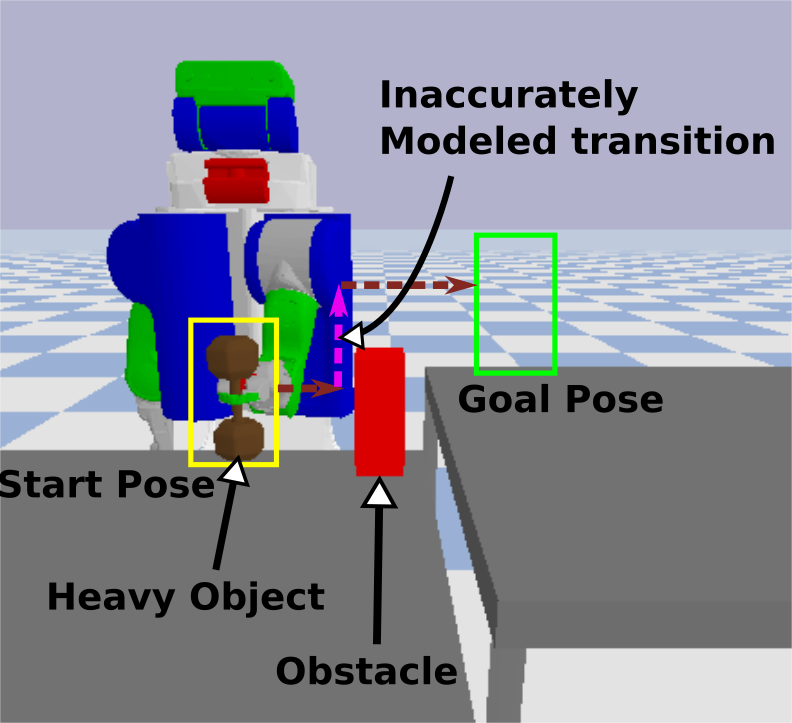
\includegraphics[width=\linewidth]{figures/cmaxpp/intro_grasp_new.png}
  \end{subfigure}
  \hspace{10mm}
  \begin{subfigure}{.4\columnwidth}
    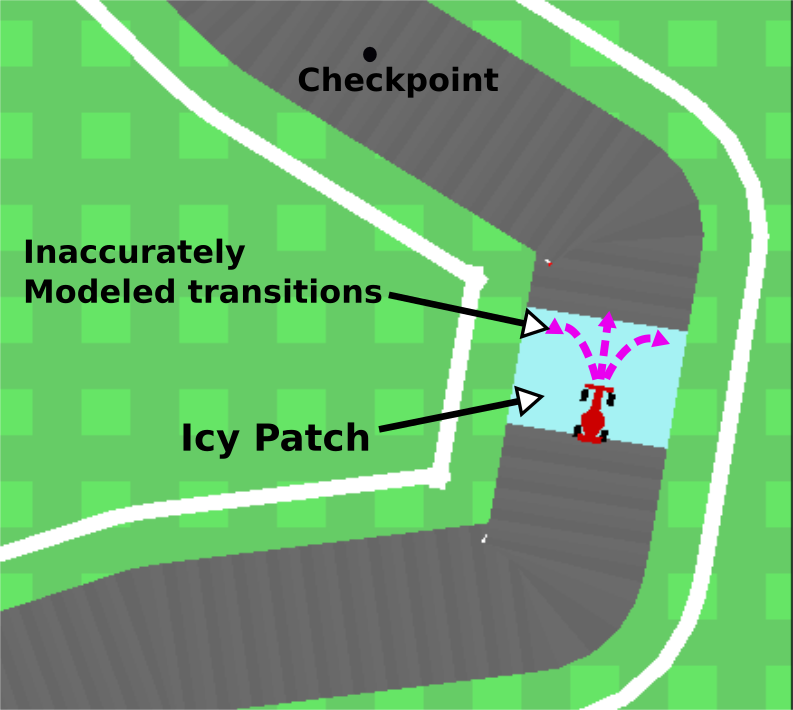
\includegraphics[width=\linewidth]{figures/cmaxpp/intro_car_new.png}
  \end{subfigure} 
  \caption{(left) PR2 lifting a heavy dumbbell, that is modeled as
    light, to a goal location that is higher than the start location
    resulting in dynamics that are inaccurately modeled (right) Mobile robot
    navigating around a track with icy patches with unknown friction parameters
    leading to the robot skidding. In both cases, any path to the goal
    needs to contain a
    transition (pink) whose dynamics are not modeled accurately.}
  \label{fig:intro}
\end{figure}

A recent planning approach, \cmax{}, introduced
in~\cite{cmax} adapts its planning strategy online to account
for any inaccuracies in the forward model without requiring any
updates to the dynamics of the model. \cmax{} achieves this online by
inflating the cost of any transition that is found to be incorrectly
modeled and replanning, thus biasing the resulting plans away from
regions where the model is inaccurate. It does so while maintaining
guarantees on completing the task, without any resets, in a finite
number of executions. However, \cmax{} requires
that there always exists a path from the current state of the robot to the goal
containing only transitions that have not yet been found to be incorrectly
modeled. This is a strong assumption on the accuracy of the model and
% is often not satisfied in several repetitive robotic tasks.
can often be violated, especially in the context of repetitive tasks.

For example, consider the task shown in Figure~\ref{fig:intro}(left)
where a robotic arm needs to repeatedly pick a heavy object, that is
incorrectly modeled as light, and place it on top of a taller table while avoiding
an obstacle. As the object is heavy, transitions that involve lifting
the object will have discrepancy between true and modeled
dynamics. However, any path from the start pose to the goal pose
requires lifting the object and thus, the resulting plan needs to
contain a transition that is incorrectly modeled. This violates the
aforementioned assumption of \cmax{}
% . \cmax{}, on this
% task,
and it ends up
inflating the cost of any transition that lifts the object,
resulting in plans that avoid lifting the object in future
repetitions. Thus, the quality of \cmax{} solution deteriorates
across repetitions and, in some cases, it even fails to complete the
task. Figure~\ref{fig:intro}(right) presents another example task
where a mobile robot is navigating around a track with icy patches
that have unknown friction parameters. Once the robot enters a patch,
any action executed results in the robot skidding, thus violating the
assumption of \cmax{} because
any path to the goal from current state will have inaccurately modeled
transitions. \cmax{}
ends up inflating the cost of all actions executed inside the icy
patch, leading to the robot being unable to find a path in future laps and
failing to complete the task. Thus, in both examples, we need a
planning approach that allows solutions to contain incorrectly modeled
transitions while ensuring that the robot reaches the goal.


In this paper we present \cmaxpp{}, an approach for interleaving
planning and execution that uses inaccurate models and leverages
experience from past executions to provably complete the task in each
repetition without any resets. Furthermore, it improves the quality of
solution across
repetitions. In contrast to \cmax{}, \cmaxpp{} requires weaker conditions to
ensure task completeness, and is provably guaranteed to
converge to a plan with optimal cost as the number of repetitions
increases.
% We achieve this by integrating model-free value
% estimates for inaccurately modeled transitions, obtained using past
% experience, within a novel model-based planning procedure using the
% inaccurate model.
The key idea behind \cmaxpp{} is to combine the conservative behavior
of \cmax{} that tries to avoid incorrectly modeled regions with
model-free Q-learning that tries to estimate and follow the optimal
cost-to-goal value function with no regard for any discrepancies
between modeled and true dynamics.
This enables \cmaxpp{} to compute plans that utilize
inaccurately modeled transitions, unlike \cmax{}. Based on this idea,
we present an algorithm
for small state
spaces, where we can do exact planning, and a practical algorithm for
large state spaces using function approximation techniques. We also propose
an adaptive version of \cmaxpp{} that intelligently switches between 
\cmax{} and \cmaxpp{} to combine the advantages of both approaches, and exhibits
goal-driven behavior in earlier repetitions and optimality in later repetitions.
The proposed algorithms are tested on simulated robotic tasks: 3D
mobile robot navigation where the track friction is incorrectly
modeled (Figure~\ref{fig:intro} right) and a 7D pick-and-place
task where the mass of the object is unknown (Figure~\ref{fig:intro} left).


\section{Related Work}
\label{sec:related-work}

A typical approach to planning in tasks with unknown parameters is to
use acquired experience from executions to update the dynamics of the
model and replan~\cite{DBLP:journals/sigart/Sutton91}. This works well
in practice for tasks where the forward model is flexible and can be
updated efficiently. However for real world tasks, the models used for
planning cannot be updated efficiently
online~\cite{DBLP:conf/iros/TodorovET12} and are often precomputed
offline using expensive
procedures~\cite{DBLP:conf/wafr/HauserBHL06}. Another line of works~\cite{DBLP:conf/iros/SaverianoYFL17,DBLP:conf/icml/AbbeelQN06}
seek to learn a residual dynamical model to account for the
inaccuracies in the initial model. However, it can take a
prohibitively large number of executions to learn the true dynamics,
especially in domains like deformable
manipulation~\cite{essahbi2012}. This precludes these approaches from
demonstrating a goal-driven behavior as we show in our experimental analysis.


Recent works such as \cmax{}~\cite{cmax}
and~\cite{DBLP:journals/ral/McConachiePMB20} pursue an alternative
approach which does not require updating the dynamics of the model or
learning a residual component. These approaches exhibit goal-driven
behavior by focusing on completing the task and not on modeling the
true dynamics accurately. While \cmax{} achieves this by inflating the
cost of any transition whose dynamics are inaccurately modeled,
\cite{DBLP:journals/ral/McConachiePMB20} present an approach that
learns a binary classifier offline that is used online to predict
whether a transition is accurately modeled or not. Although these
methods work well in practice for goal-oriented tasks, they do not
leverage experience acquired online to improve the quality of solution
when used for repetitive tasks.

% \todo[inline]{Can the following paragraph be removed? Fahad thinks it
%   is not so relevant to this work. If removed, we still need to cut
%   the draft down more to get it under 7 pages}
% Planning for repetitive robotic tasks has been an active area of
% research in the motion planning community. A typical approach is to
% pre-compute a set of complete paths into a library which is used to
% match a new query online~\cite{DBLP:conf/icra/BerensonAG12,
%   DBLP:journals/arobots/JetchevT13}. Using paths computed in previous
% repetitions to improve planning times in later
% repetitions has also been explored in previous works such
% as~\cite{DBLP:conf/socs/PhillipsCCL12,
%   DBLP:conf/icra/ColemanSMOC15}. However, these approaches assume
% access to accurate forward models and are incapable of dealing with
% inaccuracy in modeled dynamics.



Our work is closely related to approaches that integrate
model-based planning with model-free
learning. \cite{DBLP:journals/corr/abs-2005-10872} use model-based
planning in regions where the dynamics are accurately modeled and
switch to a model-free policy in regions with high
uncertainty. However, they mostly focus on perception uncertainty and
require a coarse estimate of the uncertain region prior to execution,
which is often not available for tasks with other modalities of
uncertainty like unknown inertial parameters. A very recent work
by~\cite{lagrassa2020learning} uses a
model-based planner until a model inaccuracy is detected and switches
to a model-free policy to complete the task. Similar to our approach,
they deal with general modeling errors but rely on expert
demonstrations to learn the model-free policy. In contrast, our
approach does not require any expert demonstrations and only uses the
experience acquired online to obtain model-free value estimates
that are used within planning.


Finally, our approach is also related to the field of real-time
heuristic search which tackles the problem of efficient planning in
large state spaces with bounded planning time. In this work, we
introduce a novel planner that is inspired by
LRTA*~\cite{DBLP:journals/ai/Korf90} which limits the number of
expansions in the search procedure and interleaves execution with
planning. Crucially, our planner also interleaves planning and
execution but unlike these approaches, employs model-free value
estimates obtained from past experience within the search.


% Planning and learning using inaccurate models

% Combining Model-Free Learning and Model-based planning

% Real-time heuristic search

% Local and Global function approximation techniques

\section{Problem Setup}
\label{sec:problem-setup}

Following the notation of \cite{cmax}, we consider the
deterministic shortest path problem that can be represented using  the
tuple $M = (\statespace, \actionspace, \goalspace, f, c)$ where
$\statespace$ is the state space, $\actionspace$ is the action space,
$\goalspace \subseteq \statespace$ is the non-empty set of goals,
$f:\statespace \times \actionspace \rightarrow \statespace$ is a
deterministic dynamics function, and $c:\statespace \times
\actionspace \rightarrow [0, 1]$ is the cost function. Note that we
assume that the costs lie between $0$ and $1$ but any bounded cost
function can be scaled to satisfy this assumption. Crucially, our
approach assumes that the action space $\actionspace$ is discrete, and any
goal state $g \in \goalspace$ is a cost-free termination state. The
objective of the shortest path problem is to find the least-cost path
from a given start state $s_1 \in \statespace$ to any goal state $g
\in \goalspace$ in $M$. As is typical in shortest path problems, we
assume that there exists at least one path from each state $s \in
\statespace$ to one of the goal states, and that the cost of any
transition from a non-goal state is
positive~\cite{DBLP:books/lib/Bertsekas05}. We will use $V(s)$ to
denote the state value function (a running estimate of cost-to-goal
from state $s$,) and $Q(s, a)$ to denote the
state-action value function (a running estimate of the sum of
transition cost and cost-to-goal from successor state,) for any state $s$ and action
$a$. Similarly, we will use the notation $V^*(s)$ and $Q^*(s, a)$ to
denote the corresponding optimal value functions. A value estimate is
called admissible if it underestimates the optimal value function at
all states and actions, and is called consistent if it satisfies the
triangle inequality, i.e. $V(s) \leq c(s, a) + V(f(s, a))$ and $Q(s,
a) \leq c(s, a) + V(f(s, a))$ for all $s, a$, and $V(g) = 0$ for all $g \in \goalspace$.


In this work, we focus on repetitive robotic tasks where the true
deterministic dynamics $f$ are unknown but we have access to an
approximate model described using $\Mhat = (\statespace, \actionspace,
\goalspace, \fhat, c)$ where $\fhat$ approximates the true dynamics.
In each repetition of the task, the robot acts in the environment $M$
to acquire experience over a single trajectory and reach the goal,
without access to any resets. This rules out any episodic
approach.
% The robot is reset back to the start state in next
% repetition of the task only if it was successful in the previous
% repetition.
Since the true dynamics are unknown and can only be
discovered through executions, we consider the online real-time
planning setting where the robot has to interleave planning and
execution.
In our motivating navigation example (Figure~\ref{fig:intro} right,)
the approximate model $\hat{M}$ represents a track with no icy patches
whereas the environment $M$ contains icy patches. Thus, there is a 
discrepancy between the modeled dynamics $\fhat$ and true
dynamics $f$. Following \cite{cmax}, we will refer to
state-action pairs that have inaccurately modeled dynamics as
``incorrect" transitions, and use the notation $\incorrectset
\subseteq \statespace \times \actionspace$ to denote the set of discovered
incorrect transitions. The objective in our work is for the robot to
reach a goal in each repetition, despite using an inaccurate model for
planning while improving performance, measured using the cost of
executions, across repetitions. 


\section{Approach}
\label{sec:approach}

In this section, we will describe the proposed approach \cmaxpp{}. 
First, we will present a novel planner used in \cmaxpp{} that
can exploit incorrect transitions using their model-free $Q$-value
estimates. Second, we present \cmaxpp{} and its adaptive version
for small state spaces, and establish their guarantees. Finally, we
describe a practical instantiation of \cmaxpp{} for large state spaces
leveraging function approximation techniques.

%In
%Section~\ref{sec:integrating-q-values}, we introduce a novel real-time
%heuristic search-based planner that uses model-free state-action value
%estimates within a model-based planning
%procedure. Section~\ref{sec:warm-up:-small} presents \cmaxpp{} for
%small discrete state spaces where it is feasible to maintain tabular
%value estimates and perform exact planning. Subsequently, we present
%an adaptive version of \cmaxpp{} that intelligently switches between
%\cmax{} and \cmaxpp{} to combine the advantages of both approaches in
%Section~\ref{sec:adaptive}. Finally, we extend \cmaxpp{} and adaptive
%\cmaxpp{} to large state spaces in
%Section~\ref{sec:large-state-spaces} where we resort to function
%approximation techniques for maintaining value estimates and the
%incorrect set $\incorrectset$.


\subsection{Hybrid Limited-Expansion Search Planner}
\label{sec:integrating-q-values}

During online execution, we want the robot to acquire experience
and leverage it to compute better plans. This requires a hybrid planner that
is able to incorporate value estimates obtained using past experience
in addition to model-based planning, and quickly compute the next
action to execute. To achieve this, we propose a real-time
heuristic search-based planner that performs a bounded number of
expansions and is able to utilize $Q$-value estimates for incorrect
transitions.


\begin{algorithm}[t]
  \caption{Hybrid Limited-Expansion Search}
  {\normalsize
  \begin{algorithmic}[1]
    \Procedure{$\mathtt{SEARCH}$}{$s,
      \Mhat, V, Q, \incorrectset, K$}
      \State Initialize $g(s)=0$, min-priority open list $O$, and closed list $C$
      \State Add $s$ to open list $O$ with priority $p(s) = g(s) + V(s)$
      \For{$i = 1, 2, \cdots, K$}
      	\State Pop $s_i$ from $O$
      	\If{$s_i$ is a dummy state or $s_i \in \goalspace$}
      	\State Set $s_\best \leftarrow s_i$ and go to Line~\ref{line:update}\label{line:jump}
      	\EndIf
      	\For{$a \in \actionspace$}\Comment{\textit{Expanding state $s_i$}}
      		\If{$(s_i, a) \in \incorrectset$}\Comment{\textit{Incorrect transition}}
      		\State Add a dummy state $s'$ to $O$ with priority $p(s') = g(s_i) + Q(s_i, a)$\label{line:dummy}
     		\State \textbf{continue}
      		\EndIf
      		\State Get successor $s' = \fhat(s_i, a)$
      		\State If $s' \in C$, \textbf{continue}
      		\If{$s' \in O$ and $g(s') > g(s_i) + c(s_i, a)$}
      			\State Set $g(s') = g(s_i) + c(s_i, a)$ and recompute $p(s')$
      			\State Reorder open list $O$
      		\ElsIf{$s' \notin O$}
      			\State Set $g(s') = g(s_i) + c(s_i, a)$
      			\State Add $s'$ to $O$ with priority $p(s') = g(s') + V(s')$
      		\EndIf
      	\EndFor
      	\State Add $s_i$ to closed list $C$
      \EndFor
      \State Pop $s_\best$ from open list $O$\label{line:best}
      \For{$s' \in C$}\label{line:update}
      	\State Update $V(s') \leftarrow p(s_\best) - g(s')$\label{line:update2}
      \EndFor
      \State Backtrack from $s_\best$ to $s$, and set $a_\best$ as the first action on path from $s$ to $s_\best$ in the search tree\label{line:best-action}
		%\State Set $a_\best$ as the first action on path from $s$ to $s_\best$
		      
      \Return{$a_\best$}
    \EndProcedure
  \end{algorithmic}}
  \label{alg:hybrid-limited-expansion-search}
\end{algorithm}

The planner is presented in
Algorithm~\ref{alg:hybrid-limited-expansion-search}. Given the current
state $s$, the planner constructs a lookahead search tree using at
most $K$ state expansions. For each expanded state $s_i$, if any
outgoing transition has been flagged as incorrect based on experience, i.e. $(s_i, a) \in \incorrectset$,
then the planner creates a dummy state with priority computed using
the model-free $Q$-value estimate of that transition
(Line~\ref{line:dummy}). Note that we create a dummy state because the
model $\Mhat$ does not know the true successor of an incorrect transition.
For
the transitions that are correct, we obtain successor states
using the approximate model $\Mhat$. This ensures that we rely on the
inaccurate model only for transitions that are not known to be
incorrect.
At any stage, if a dummy state is expanded then we need to terminate
the search as the model $\Mhat$ does not know any of its successors,
in which case we set the best state $s_\best$ as the dummy state (Line~\ref{line:jump}).
% then the lookahead tree
% construction terminates with the best state $s_\best$ as the dummy
% state.
Otherwise, we choose $s_\best$ as the best state (lowest priority)
among the
leaves of the search tree after $K$ expansions (Line~\ref{line:best}). Finally, the best
action to execute at the current state $s$ is computed as the first
action along the path from $s$ to $s_\best$ in the search tree (Line~\ref{line:best-action}). The
planner also updates state value estimates $V$ of all expanded states
using the priority of the best state $p(s_\best)$ to make the
estimates more accurate (Lines~\ref{line:update}
and~\ref{line:update2}) similar to RTAA*~\cite{DBLP:conf/atal/KoenigL06}.


The ability of our planner to exploit incorrect transitions using
their model-free $Q$-value estimates, obtained from past experience,
distinguishes it from
% \cmax{} which primarily uses
% the penalized model for planning and uses past experience only to
% update the incorrect set $\incorrectset$.
real-time search-based planners such as
LRTA*~\cite{DBLP:journals/ai/Korf90} which cannot utilize model-free
value estimates during planning.
This enables \cmaxpp{} to
result in plans that utilize incorrect transitions if they enable the
robot to get to the goal with lower cost.

\subsection{CMAX++ in  Small State Spaces}
\label{sec:warm-up:-small}

\cmaxpp{} in small state spaces is simple and easy-to-implement as it
is feasible to maintain value estimates in a table for all states and
actions and to explicitly maintain a running set of incorrect
transitions with fast lookup without resorting to function
approximation techniques.


\begin{algorithm}[t]
	\caption{\cmaxpp{} and \textcolor{blue}{\acmaxpp{}} in small state spaces}
	\begin{algorithmic}[1]
		\Require{Model $\Mhat$, start state $s$, initial value estimates $V$, $Q$, number of expansions $K$, $t\leftarrow 1$, incorrect set $\incorrectset \leftarrow \{\}$, Number of repetitions $N$, \textcolor{blue}{Sequence $\{\alpha_i \geq 1\}_{i=1}^N$, initial penalized value estimates $\Vtilde = V$, penalized model $\Mtilde \leftarrow \Mhat$}}
		\For{each repetition $i=1,\cdots, N$}
		\State $t \leftarrow 1$, $s_1 \leftarrow s$
		\While{$s_t \notin \goalspace$}
			\State Compute $a_t = \mathtt{SEARCH}(s_t, \Mhat, V, Q, \incorrectset, K)$ \label{line:cmaxpp-action}
			\textcolor{blue}{
			\State Compute $\tilde{a}_t = \mathtt{SEARCH}(s_t, \Mtilde, \Vtilde, Q, \{\}, K)$\label{line:cmax-action}
			\State If $\Vtilde(s_t) \leq \alpha_i V(s_t)$, assign $a_t = \tilde{a}_t$\label{line:switch}
			}
			\State Execute $a_t$ in environment to get $s_{t+1} = f(s_t, a_t)$
			\If{$s_{t+1} \neq \fhat(s_t, a_t)$}
				\State Add $(s_t, a_t)$ to the set: $\incorrectset \leftarrow \incorrectset \cup \{(s_t, a_t)\}$
				\State Update: $Q(s_t, a_t) = c(s_t, a_t) + V(s_{t+1})$
				\textcolor{blue}{
				\State Update penalized model $\Mtilde \leftarrow \Mtilde_{\incorrectset}$
				}
			\EndIf
			\State $t \leftarrow t + 1$
		\EndWhile
		\EndFor
	\end{algorithmic}
	\label{alg:small-state-spaces}
\end{algorithm}

The algorithm is presented in Algorithm~\ref{alg:small-state-spaces}
(only the text in black.) \cmaxpp{} maintains a running estimate of the set
of incorrect transitions $\incorrectset$, and updates the set
whenever it encounters an incorrect state-action pair during
execution. Crucially, unlike \cmax{}, it maintains a $Q$-value estimate
for the incorrect transition that is used during planning in
Algorithm~\ref{alg:hybrid-limited-expansion-search}, thereby enabling
the planner to compute paths that contain incorrect transitions. It is
also important to note that, like \cmax{}, \cmaxpp{} never updates the
dynamics of the model. However, instead of
using the penalized model for planning as \cmax{} does, \cmaxpp{} uses the initial
model $\Mhat$, and utilizes both model-based planning and model-free
$Q$-value estimates to replan a path from the current state to a goal.

The downside of \cmaxpp{} is that estimating $Q$-values from online
executions can be inefficient as it might take many executions before
we obtain an accurate $Q$-value estimate for an incorrect
transition. This has been extensively studied in the past and is a
major disadvantage of model-free
methods~\cite{DBLP:conf/colt/SunJKA019}. As a result of this
inefficiency, \cmaxpp{} lacks the goal-driven behavior of \cmax{} in
early repetitions of the task, despite achieving optimal behavior in
later repetitions. In the next section, we present an adaptive version
of \cmaxpp{} (\acmaxpp{}) that combines the goal-driven behavior of \cmax{} with
the optimality of \cmaxpp{}.



\subsection{Adaptive Version of CMAX++}
\label{sec:adaptive}

% The idea behind Adaptive-\cmaxpp{} (or, \acmaxpp{}) is to intelligently switch between
% \cmax{} and \cmaxpp{}. Intuitively, we would want to use \cmax{} in
% the earlier repetitions as it quickly finds alternative path to a goal
% without wasting executions on estimating $Q$-values of incorrect
% transitions accurately. On the other hand, we want the planner to
% compute plans with lower costs, potentially containing incorrect
% transitions, in later repetitions and thus using \cmaxpp{} would be
% ideal.

\subsubsection{Background on CMAX}
\label{sec:background-cmax}
Before we describe \acmaxpp{}, we will start by summarizing
\cmax{}. For more details, refer 
to~\cite{cmax}.
At each time step $t$ during execution, \cmax{} maintains a running
estimate of the incorrect set $\incorrectset$, and constructs a
penalized model specified by the tuple $\Mtilde_\incorrectset =
(\statespace, \actionspace, \goalspace, \fhat,
\ctilde_{\incorrectset})$ where the cost function
$\ctilde_{\incorrectset}(s, a) = |\statespace|$ if $(s, a) \in
\incorrectset$, else $\ctilde_{\incorrectset}(s, a) = c(s, a)$. In
other words, the cost of any transition found to be incorrect is
set high (or inflated) while the cost of other transitions are the
same as in $\Mhat$.
\cmax{} uses the penalized model $\Mtilde_{\incorrectset}$ to plan a path from the
current state $s_t$ to a goal state. Subsequently, \cmax{} executes
the first action $a_t$ along the path and observes if the true
dynamics and model dynamics differ on the executed action. If so, the
state-action pair $(s_t, a_t)$ is appended to the incorrect set
$\incorrectset$  and the penalized model $\Mtilde_{\incorrectset}$ is updated.
\cmax{} continues to do this at every
timestep until the robot reaches a goal state.

Observe that the inflation of cost for any incorrect state-action pair
biases the planner to ``explore" all other state-action pairs that are
not yet known to be incorrect before it plans a path using an
incorrect transition. This induces a goal-driven behavior in the
computed plan that enables \cmax{} to quickly find an alternative path
and not waste executions learning the true dynamics

\subsubsection{A-CMAX++}
\label{sec:acmaxpp}
\acmaxpp{} is presented in
Algorithm~\ref{alg:small-state-spaces} (black and blue text.)
\acmaxpp{} maintains a running estimate of incorrect set
$\incorrectset$ and constructs the penalized model $\Mtilde$ at each
time step $t$, similar to \cmax{}. For any state at time step $t$, we
first compute the best action $a_t$ based on the approximate model
$\Mhat$ and the model-free $Q$-value estimates
(Line~\ref{line:cmaxpp-action}.) In addition, we also compute the best
action $\tilde{a}_t$ using the penalized model $\Mtilde$, similar to
\cmax{}, that inflates the cost of any incorrect transition
(Line~\ref{line:cmax-action}.) The crucial step in \acmaxpp{}
is Line~\ref{line:switch} where we compare the penalized value
$\Vtilde(s_t)$ (obtained using penalized model $\Mtilde$) and the
non-penalized value $V(s_t)$ (obtained using approximate model $\Mhat$
and $Q$-value estimates.) Given a sequence $\{\alpha_i \geq 1\}$ for
repetitions $i=1,\cdots,N$ of the task, if $\Vtilde(s_t) \leq
\alpha_iV(s_t)$, then we execute action $\tilde{a}_t$, else we execute
$a_t$. This implies that if the cost incurred by following \cmax{}
actions in the future is within $\alpha_i$ times the cost incurred by
following \cmaxpp{} actions, then we prefer to execute \cmax{}.

If
the sequence $\{\alpha_i\}$ is chosen to be non-increasing such that
$\alpha_1 \geq \alpha_2 \cdots \geq \alpha_N \geq 1$, then we can observe that
\acmaxpp{} has the desired anytime-like behavior. It remains goal-driven in
early repetitions, by choosing \cmax{} actions, and
converges to optimal behavior in later repetitions, by choosing
\cmaxpp{} actions. Further, the
executions needed to obtain accurate $Q$-value estimates is
distributed across repetitions ensuring that \acmaxpp{} does
not have poor performance in any single repetition. Thus,
\acmaxpp{} combines the advantages of both \cmax{} and \cmaxpp{}.


\subsection{Theoretical Guarantees}
\label{sec:guarantees}

We will start with formally stating the assumption needed by
\cmax{} to ensure completeness:
\begin{assumption}[\cite{cmax}]
	Given a penalized model $\Mtilde_{\incorrectset_t}$ and the
        current state $s_t$ at any time step $t$, there always exists
        at least one path from $s_t$ to a goal that does not contain
        any state-action pairs $(s, a)$ that are known to be
        incorrect, i.e. $(s, a) \in \incorrectset_t$.  
        \label{assumption:cmax}      
\end{assumption}
Observe that the above assumption needs to be valid at every time step
$t$ before the robot reaches a goal and thus, can be hard to satisfy.
% In contrast, our proposed approach \cmaxpp{} requires a weaker set of
% conditions for completeness that are easier to satisfy and do not
% depend on execution.
Before we state the theoretical guarantees for \cmaxpp{}, we
need the following assumption on the approximate model $\Mhat$ that is
used for planning:
\begin{assumption}
	The optimal value function $\hat{V}^*$ using the dynamics of
        approximate model $\Mhat$ underestimates the optimal value
        function $V^*$ using the true dynamics of $M$ at all states,
        i.e. $\Vhat^*(s) \leq V^*(s)$ for all $s \in
        \statespace$.    
	\label{assumption:cmaxpp}
\end{assumption}
In other words, if there exists a path from any state $s$ to a goal
state in the environment $M$, then there exists a path with the same
or lower cost from $s$ to a goal in the approximate model $\Mhat$. In
our motivating example of pick-and-place (Figure~\ref{fig:intro}
left,) this assumption is satisfied if the object is modeled as light
in $\Mhat$, as the object being heavy in reality can only increase the cost. 
% Similarly in the navigation example
% (Figure~\ref{fig:intro} right,) it is satisfied if the track in the
% model $\Mhat$ has no icy patches as the robot does not skid and can
% reach the goal with lower costs.
This assumption was also considered in previous
works such as~\cite{DBLP:conf/aaai/Jiang18} and is known as the
\textit{Optimistic Model Assumption}.

\subsubsection{Significance of Optimistic Model Assumption}
\label{sec:sign-optim-model}

To understand the significance of the optimistic model assumption, it
is important to note that completeness guarantees usually require the
use of admissible and consistent value estimates, i.e. estimates that
always underestimate the true cost-to-goal values. This requirement
needs to hold every time we plan (or replan) to ensure that we never
discard a path as being expensive in terms of cost, when it is cheap
in reality.


All our guarantees assume that the initial value estimates are
consistent and admissible, but to ensure that they always remain
consistent and admissible throughout execution, we need the optimistic
model assumption. This assumption ensures that updating value
estimates by planning in the model $\Mhat$ always results in estimates
that are admissible and consistent. In other words, the optimal value
function (which we obtain by doing full state space planning in
$\Mhat$) of the model $\Mhat$ always underestimates the optimal value
function of the environment $M$ at all states $s \in \statespace$.


A very intuitive way to understand the assumption is to imagine a
navigation task where the robot is navigating from a start to goal in
the presence of obstacles. In this example, the optimistic model
assumption requires that the model should never place an obstacle in a
location when there isn't an obstacle in the environment at the same
location. However, if there truly is an obstacle at some location,
then the model can either have an obstacle or not have one at the same
location. Put simply, an agent that is planning using the model should
never be ``pleasantly surprised" by what it sees in the
environment. Several other intuitive examples are presented
in~\cite{DBLP:conf/aaai/Jiang18} and we recommend the reader to look
at them for more intuition.

%This is a weaker assumption than Assumption~\ref{assumption:cmax} 
%which needs to be
%satisfied at every time step $t$ during execution, while
%Assumption~\ref{assumption:cmaxpp} needs to hold for the approximate
%model we start with.

We can now state the following guarantees:
%\begin{theorem}[Completeness]
%	Assume Assumption~\ref{assumption:cmaxpp} holds, and if the
%        initial value estimates $V, Q$ are admissible and consistent,
%        then using either \cmaxpp{} or \acmaxpp{} in
%        Algorithm~\ref{alg:small-state-spaces} the robot is guaranteed
%        to reach a goal state in at most $|\statespace|^3$ time steps
%        in each repetition. Instead, if
%        Assumption~\ref{assumption:cmax} holds then using
%        \acmaxpp{} with a large enough $\alpha_i$ for any repetition
%        $i$ (typically true for early repetitions) in
%        Algorithm~\ref{alg:small-state-spaces}, the robot is        
%        guaranteed to reach a goal state in at most $|\statespace|^2$
%        time steps, and using \cmaxpp{}, it is guaranteed to reach a 
%        goal state
%        in at most $|\statespace|^3$ time steps in each repetition.       
%	\label{theorem:completeness}
%\end{theorem}
\begin{theorem}[Completeness]
	Assume the initial value estimates $V, Q$ are admissible and consistent. Then we have,
	\begin{enumerate}
		\item If Assumption~\ref{assumption:cmaxpp} holds then using either \cmaxpp{} or \acmaxpp{}, the robot is guaranteed to reach a goal state in at most $|\statespace|^3$ time steps in each repetition.
		\item If Assumption~\ref{assumption:cmax} holds then
                  (a) using \acmaxpp{} with a large enough $\alpha_i$
                  in any repetition $i$ (typically true for early
                  repetitions,) the robot is guaranteed to reach a
                  goal state in at most $|\statespace|^2$ time steps,
                  and (b) using \cmaxpp{}, it is guaranteed to reach a goal state in at most $|\statespace|^3$ time steps in each repetition
	\end{enumerate}       
	\label{theorem:completeness}
      \end{theorem}
      \begin{proof}[Proof Sketch]
	To prove completeness, first we need to note that the $Q$-update in
\cmaxpp{} always ensures that the $Q$-value estimates remain
consistent and admissible as long as the state value estimates remain
consistent and admissible. We have already seen why the optimistic
model assumption ensures that the state value estimates always remain
consistent and admissible. Thus, we can use Theorem~3 from
RTAA*~\cite{DBLP:conf/atal/KoenigL06} in conjunction with the
optimistic model assumption to ensure completeness. Note that if the
model is inaccurate everywhere, then our planner reduces to doing
$K=1$ expansions at every time step and acts similar to $Q$-learning,
which is also guaranteed to be complete with admissible and consistent
estimates~\cite{DBLP:conf/aaai/KoenigS93}. The worst case bound of
$|\statespace|^3$ steps is taken directly from the upper bound on
$Q$-learning from~\cite{DBLP:conf/aaai/KoenigS93}. The above arguments
are true for both \cmaxpp{} and \acmaxpp{}. Note that for \acmaxpp{}
if all paths to the goal contains an incorrect transition then the
penalized value estimate $\Vtilde(s) > \alpha V(s)$ for any finite
$\alpha$ and thus, will fall back on \cmaxpp{}.


For the second part of the theorem, the assumption of \cmax{} (we will
refer this as \textit{optimistic penalized model assumption}) in
conjunction with RTAA* guarantee again ensures completeness for
\cmaxpp{} and \acmaxpp{}. To see this, observe that the optimistic
penalized model assumption ensures that the value estimates are always
admissible and consistent w.r.t the true penalized model
($\Mtilde_\incorrectset$ where $\incorrectset$ contains all the
incorrect transitions) and from the assumption, we know that there
exists a path to the goal in the true penalized model. Hence,
\cmaxpp{} and \acmaxpp{} are bound to find this path.


\cmaxpp{} again utilizes the worst case bounds of $Q$-learning under
the optimistic penalized assumption as well and attains an upper bound
of $|\statespace|^3$ steps. However, \acmaxpp{} with a sufficiently
large $\alpha_i$ for any repetition $i$ acts similar to \cmax{}, and
thereby can utilize the worst case bounds of LRTA* (which is simply
RTAA* with $K=1$ expansions) from~\cite{DBLP:conf/aaai/KoenigS93}
giving an upper bound of $|\statespace|^2$ time steps. This shows the
advantage of \acmaxpp{} over \cmaxpp{}, especially in earlier
repetitions when the incorrect set $\incorrectset$ is small (thus,
making the optimistic penalized model assumption hold,) and $\alpha_i$
is large.
        \end{proof}
%In addition to the above completeness guarantee, we can also prove the
%following guarantee for \cmaxpp{}:
\begin{theorem}[Asymptotic Convergence]
	Assume Assumption~\ref{assumption:cmaxpp} holds, and that the
        initial value estimates $V, Q$ are admissible and
        consistent. For sufficiently large number of repetitions $N$,
        there exists an integer $j \leq N$ such that the robot follows
        a path with the optimal cost to the goal using \cmaxpp{} in
        Algorithm~\ref{alg:small-state-spaces} in repetitions $i \geq
        j$.        
	\label{theorem:convergence}
\end{theorem}
\begin{proof}[Proof Sketch]
	The asymptotic convergence proof completely relies on the asymptotic
convergence of $Q$-learning~\cite{DBLP:conf/aaai/KoenigS93} and
asymptotic convergence of LRTA*~\cite{DBLP:journals/ai/Korf90} to
optimal value estimates. The proof again crucially relies on the fact
that the value estimates always remain admissible and consistent,
which is ensured by the optimistic model assumption. Note that the
optimistic penalized model assumption is not enough to guarantee
asymptotic convergence to the optimal cost in $M$ as we penalize
incorrect transitions. However, it is possible to show that under the
optimistic penalized model assumption both \cmaxpp{} and \acmaxpp{}
converge to the optimal cost in the true penalized model
$\Mtilde_\incorrectset$ where $\incorrectset$ contains all incorrect
transitions.
        \end{proof}

It is important to note that
the conditions required for Theorem~\ref{theorem:completeness}
are weaker than the conditions required for completeness of
\cmax{}. Firstly,
if either Assumption~\ref{assumption:cmax} or
Assumption~\ref{assumption:cmaxpp} holds then \cmaxpp{} can be shown
to be complete, but \cmax{} is guaranteed to be complete only under
Assumption~\ref{assumption:cmax}.
Furthermore,
Assumption~\ref{assumption:cmaxpp} only needs to hold
for the approximate model $\Mhat$ we start with, whereas
Assumption~\ref{assumption:cmax} needs to be satisfied for every penalized model $\Mtilde$ constructed at any time
step $t$ during execution.


%In practice, we observe that the number of time steps taken by \cmaxpp{} to reach a goal has a much smaller dependence on the size of
%state space compared to the worst-case bound in
%Theorem~\ref{theorem:completeness}, especially if the initial value
%estimates are close to the optimal value estimates for the approximate
%model $\Mhat$ which can be computed offline.

\subsection{Large State Spaces}
\label{sec:large-state-spaces}

\begin{algorithm}[t]
	\caption{\cmaxpp{} in large state spaces}
	\begin{algorithmic}[1]
		\Require{Model $\Mhat$, start state $s$, value function approximators $V_\theta$, $Q_\zeta$, number of expansions $K$, $t\leftarrow 1$, Discrepancy threshold $\xi$, Radius of hypersphere $\delta$, Set of hyperspheres $\incorrectset^\xi \leftarrow \{\}$, Number of repetitions $N$, Batch size $B$, State buffer $\buffer_S$, Transition buffer $\buffer_{SA}$, Learning rate $\eta$, Number of updates $U$}
		\For{each repetition $i=1,\cdots, N$}
		\State $t \leftarrow 1$, $s_1 \leftarrow s$
		\While{$s_t \notin \goalspace$}
			\State Compute $a_t = \mathtt{SEARCH}(s_t, \Mhat, V_\theta, Q_\zeta, \incorrectset^\xi, K)$
			\State Execute $a_t$ in environment to get $s_{t+1} = f(s_t, a_t)$
			\If{$d(s_{t+1}, \fhat(s_t, a_t)) > \xi$}
				\State Add hypersphere: $\incorrectset^\xi \leftarrow \incorrectset^\xi \cup \{\mathsf{sphere}(s_t, a_t, \delta)\}$\label{line:hypersphere}
				%\State Update: $Q(s_t, a_t) = c(s_t, a_t) + V(s_{t+1})$
			\EndIf
			\State Add $s_t$ to $\buffer_S$, and $(s_t, a_t, s_{t+1})$ to $\buffer_{SA}$
			\For{$u=1,\cdots, U$}\Comment{\textit{Approximator updates}}\label{line:approximation_updates}
			\State $\mathtt{Q\_UPDATE}(Q_\zeta, V_\theta, \buffer_{SA})$
			\State $\mathtt{V\_UPDATE}(V_\theta, Q_\zeta, \buffer_S, \incorrectset^\xi)$
			\EndFor
%			\State $\mathtt{UPDATE}(V_\theta, Q_\zeta, \incorrectset^\xi, \buffer_S, \buffer_{SA})$
			\State $t \leftarrow t + 1$
		\EndWhile
		\EndFor
%		\Procedure{$\mathtt{UPDATE}$}{$V_\theta, Q_\zeta, \incorrectset^\xi, \buffer_S, \buffer_{SA}$}
%			\For{$n=1,\cdots,U$}
%				\State Sample $B$ transitions from $\buffer_{SA}$ with replacement
%				\State Construct training set $\trainingset_Q = \{((s_i, a_i), Q(s_i, a_i))\}$ for each sampled transition $(s_i, a_i, s_i')$ and compute $Q(s_i, a_i) = c(s_i, a_i) + V_\theta(s_i')$
%				\State Update: $\zeta \leftarrow \zeta - \eta \nabla_\zeta \loss_Q(Q_\zeta, \trainingset_Q)$
%				\State Sample $B$ states from $\buffer_S$ with replacement
%				\State Call $\mathtt{SEARCH}$ for each sampled $s_i$ to get all states on closed list $s_i'$ and their corresponding value updates $V(s_i')$ to construct training set $\trainingset_V = \{(s_i', V(s_i')\}$
%				\State Update: $\theta \leftarrow \theta - \eta \nabla_\theta \loss_V(V_\theta, \trainingset_V)$
%			\EndFor
%		\EndProcedure
	\Procedure{$\mathtt{Q\_UPDATE}$}{$Q_\zeta, V_\theta, \buffer_{SA}$}\label{line:q-update}
		\State Sample $B$ transitions from $\buffer_{SA}$ with replacement\label{line:transition-sample}
		\State Construct training set $\trainingset_Q = \{((s_i, a_i), Q(s_i, a_i))\}$ for each sampled transition $(s_i, a_i, s_i')$ and compute $Q(s_i, a_i) = c(s_i, a_i) + V_\theta(s_i')$
		\State Update: $\zeta \leftarrow \zeta - \eta \nabla_\zeta \loss_Q(Q_\zeta, \trainingset_Q)$
	\EndProcedure
	\Procedure{$\mathtt{V\_UPDATE}$}{$V_\theta, Q_\zeta, \buffer_S, \incorrectset^\xi$}\label{line:v-update}
		\State Sample $B$ states from $\buffer_S$ with replacement\label{line:state-sample}
		\State Call $\mathtt{SEARCH}(s_i, \Mhat, V_\theta, Q_\zeta, \incorrectset^\xi, K)$ for each sampled $s_i$ to get all states on closed list $s_i'$ and their corresponding value updates $V(s_i')$ to construct training set $\trainingset_V = \{(s_i', V(s_i')\}$
		\State Update: $\theta \leftarrow \theta - \eta \nabla_\theta \loss_V(V_\theta, \trainingset_V)$
	\EndProcedure
	\end{algorithmic}
	\label{alg:large-state-spaces}
\end{algorithm}


In this section, we present a practical instantiation of \cmaxpp{} for
large state spaces where it is infeasible to maintain tabular value
estimates and the incorrect set $\incorrectset$ explicitly. Thus, we
leverage function approximation techniques to maintain these
estimates. Assume that there exists a 
metric $d$ under which $\statespace$ is bounded. We relax the definition
of incorrect set using this metric to define $\incorrectset^\xi$ as
the set of all $(s, a)$ pairs such that $d(f(s, a), \fhat(s, a)) >
\xi$ where $\xi \geq 0$. Typically, we chose $\xi$ to allow for small
modeling discrepancies that can be compensated by a low-level path
following controller.

\cmaxpp{} in large state spaces is presented in
Algorithm~\ref{alg:large-state-spaces}. The algorithm closely follows
\cmax{} for large state spaces presented in~\cite{cmax}. The
incorrect set $\incorrectset^\xi$ is maintained using sets of
hyperspheres with each set corresponding to a discrete
action. Whenever the agent executes an incorrect state-action $(s,
a)$, \cmaxpp{} adds a hypersphere centered at $s$ with radius
$\delta$, as measured using metric $d$, to the incorrect set
corresponding to action $a$. In future
planning, any state-action pair $(s', a')$ is declared incorrect if
$s'$ lies inside any of the hyperspheres in the incorrect set
corresponding to action $a'$.
After each execution, \cmaxpp{} proceeds to update the value
function approximators (Line~\ref{line:approximation_updates}) by
sampling previously executed transitions and visited states from
buffers and performing gradient descent steps
(Procedures~\ref{line:q-update} and~\ref{line:v-update}) using mean
squared loss
functions given by $\loss_Q(Q_\zeta, \trainingset_Q) =
                                     \frac{1}{2|\trainingset_Q|}\sum_{(s_i,
                                     a_i) \in \trainingset_Q} (Q(s_i,
                                     a_i) - Q_\zeta(s_i, a_i))^2$ and $\loss_V(V_\theta, \trainingset_V) = \frac{1}{2|\trainingset_V|}\sum_{s_i \in \trainingset_V} (V(s_i) - V_\theta(s_i))^2$.

By using hyperspheres, \cmaxpp{} ``covers" the set of incorrect
transitions, and enables fast lookup using KD-Trees in the state
space. Like
Algorithm~\ref{alg:small-state-spaces}, we never update the
approximate model $\Mhat$ used for planning. However, unlike
Algorithm~\ref{alg:small-state-spaces}, we update the value estimates
for sampled previous transitions and states
(Lines~\ref{line:transition-sample} and~\ref{line:state-sample}). This ensures that the
global function approximations used to maintain value estimates
$V_\theta, Q_\zeta$ have good generalization beyond the current state
and action. Algorithm~\ref{alg:large-state-spaces} can also be extended in a similar fashion as Algorithm~\ref{alg:small-state-spaces} to include \acmaxpp{} by maintaining a penalized value function approximation and updating it using gradient descent.


\section{Experiments}
\label{sec:experiments}

We test the efficiency of \cmaxpp{} and \acmaxpp{} on
simulated robotic tasks emphasizing their performance in each
repetition of the task, and improvement across
repetitions\footnote{The code to reproduce our experiments can be 
found at \url{https://github.com/vvanirudh/CMAXPP}.}. In each
task, we start the next repetition only if the robot reached a goal in
previous repetition.


\subsection{3D Mobile Robot Navigation with Icy Patches}
\label{sec:simulated-3d-mobile}

In this experiment, the task is for a mobile robot with Reed-Shepp
dynamics~\cite{reeds1990} to navigate around a track $M$ with icy
patches (Figure~\ref{fig:intro} right.) This
can be represented as a planning problem in 3D discrete state space
$\statespace$ with any state represented using the tuple $(x, y,
\theta)$ where $(x, y)$ is the 2D position of the robot and $\theta$
describes its heading. The XY-space is discretized into $100 \times
100$ grid and the $\theta$ dimension is discretized into $16$
cells. We construct a lattice
graph~\cite{DBLP:journals/jfr/PivtoraikoKK09} using $66$ motion
primitives that are pre-computed offline respecting the differential
constraints on the motion of the robot. The model $\Mhat$ used for
planning contains the same track as $M$ but without any icy patches,
thus the robot discovers transitions affected by icy patches only
through executions.

\begin{figure}[t]
  \centering
  \includegraphics[width=0.9\linewidth]{figures/cmaxpp/car_racing_bar_add.pdf}
  \caption{Number of steps taken to finish a lap averaged across 10 instances each with $5$ icy patches placed randomly around the track. The number above each bar reports the number of instances in which the robot was successful in finishing the respective lap within $10000$ time steps.}
  \label{fig:car_racing}
\end{figure}

Since the state space is small, we use
Algorithm~\ref{alg:small-state-spaces} for \cmaxpp{} and
\acmaxpp{}. For \acmaxpp{}, we use a non-increasing sequence with
$\alpha_i = 1 + \beta_i$ where $\beta_1 = 100$ and $\beta_i$ is
decreased by 2.5 after every $5$ repetitions (See Appendix for more details on choosing the sequence.) We
compare both algorithms with \cmax{}. For all the approaches, we
perform $K=100$ expansions. Since
the motion primitives are computed offline using an expensive
procedure, it is not feasible to update the dynamics of model $\Mhat$
online and hence, we do not compare with any model learning baselines. We
also conducted several experiments with model-free Q-learning, and found that it
performed poorly requiring a very large number of executions and finishing
only 10 laps in the best case. Hence, we do not include it in our
results shown in Figure~\ref{fig:car_racing}.

\cmax{} performs
well in the early laps computing paths with lower costs compared to
\cmaxpp{}. However, after a few laps the robot using \cmax{} gets
stuck within an icy patch and does not make any more progress. Observe
that when the robot is inside the icy patch,
Assumption~\ref{assumption:cmax} is violated and \cmax{} ends up
inflating all transitions that take the robot out of the patch leading
to the robot finishing $200$ laps in $2$ out of $10$
instances. \cmaxpp{}, on the other hand, is suboptimal in the initial
laps, but converges to paths with lower costs in later
laps. More importantly, the robot using \cmaxpp{} manages to finish
$200$ laps in all $10$ instances. \acmaxpp{} also successfully
finishes $200$ laps in all $10$ instances. However, it 
%performs as
%well as \cmax{} in the initial laps and achieves paths with lower costs like
%\cmaxpp{} in the later laps.
outperforms both \cmax{} and \cmaxpp{} in all laps by intelligently switching between them achieving goal-driven behavior in early laps and optimal behavior in later laps.
Thus, \acmaxpp{} combines the
advantages of \cmax{} and \cmaxpp{}.



\subsection{7D Pick-and-Place with a Heavy Object}
\label{sec:simulated-7d-pick}

%\begin{table*}[t]
%  \centering
%  \small
%  \begin{tabular}{|c|c|c|c|c|c|}
%    \hline
%    \textit{Repetition$\rightarrow$} & $1$ & $5$ & $10$ & $15$ & $20$ \\
%    \hline
%    \textbf{\cmax{}} & $\mathbf{17.8 \pm 3.4 (5)}$& $13.6 \pm 0.5 (3)$ & $18 \pm
%                                                     0(1)$&$15 \pm 0
%                                                              (1)$ &
%    $15 \pm 0(1)$\\
%    \hline
%    \textbf{\cmaxpp{}} & $\mathbf{17 \pm 4.9(5)}$ & $14.2 \pm 3.3(5)$ & $\mathbf{10.6 \pm 0.3(5)}$
%                                  & $\mathbf{11 \pm 0(5)}$ & $\mathbf{10.8 \pm 0.1(5)}$ \\
%    \hline
%    \textbf{\acmaxpp{}} & $\mathbf{17.8 \pm 3.4(5)}$ & $\mathbf{11.6 \pm 0.7(5)}$ & $17 \pm 6(5)$
%                                  & $\mathbf{10.4 \pm 0.3(5)}$ & $\mathbf{10.6 \pm 0.4(5)}$ \\
%    \hline
%    \textbf{Model KNN} & $40.6 \pm 7.3(5)$ & $12.8 \pm 1.3(5)$ & $29.6 \pm
%                                                      16.1(5)$ &
%                                                                   $15.8\pm
%                                                                   2.9(5)$
%                                         & $12.4 \pm 1.4(5)$\\
%    \hline
%    \textbf{Model NN} & $56 \pm 16.2(5)$& $208.2 \pm 92.1(4)$ & $124.5 \pm
%                                                     81.6(2)$ & $28
%                                                                  \pm
%                                                                  7.7(2)$
%                                         & $37.5 \pm 20.1(2)$\\
%    \hline
%    \textbf{Q-learning} & $172.4\pm 75(5)$& $23.2\pm 10.3(4)$ & $26.5 \pm
%                                                           6.7(4)$ &
%                                         $18 \pm 2.8(4)$& $10.2 \pm 0.6(4)$ \\
%    \hline
%  \end{tabular}
%  \caption{Number of steps taken to reach the goal in $7$D
%    pick-and-place experiment for $5$ instances each with random start
%    and obstacle locations for $20$ repetitions. We present mean
%    and standard error for each repetition and approach \textit{only among}
%    instances in which the robot reached the goal within $500$
%    timesteps with the number of such instances given in parenthesis.}
%  \label{tab:pick-and-place}
%\end{table*}

\begin{table*}[t]
  \centering
  {\scriptsize
  \setlength\tabcolsep{3pt}
  \begin{tabular}{|c|c|c|c|c|c|c|c|c|c|c|}
    \hline
    \textit{Repetition$\rightarrow$} & \multicolumn{2}{c|}{${1}$} &
                                                                  \multicolumn{2}{c|}{${5}$} & \multicolumn{2}{c|}{${10}$} & \multicolumn{2}{c|}{${15}$} & \multicolumn{2}{c|}{${20}$} \\
    \cline{2-11}
    & \textit{Steps} & \textit{Success} & \textit{Steps} & \textit{Success} & \textit{Steps} & \textit{Success} &
                                                                     \textit{Steps}
                         & \textit{Success} &
                                                       \textit{Steps} & \textit{Success} \\
    \hline
    \cmax{} & $\mathbf{17.8 \pm 3.4}$ & $100\%$& $13.6 \pm 0.5$ & $60\%$ & $18 \pm
                                                     0$ & $20\%$ & $15
                                                                   \pm
                                                                   0$
                         & $20\%$ &
    $15 \pm 0$ & $20\%$\\
    \hline
    \cmaxpp{} & $\mathbf{17 \pm 4.9}$ & $100\%$ & $14.2 \pm 3.3$ &
                                                                   $100\%$
                                                                                                                                                   & $\mathbf{10.6 \pm 0.3}$ & $100\%$
                                  & $\mathbf{11 \pm 0}$ &  $100\%$ & $\mathbf{10.8 \pm
                                                            0.1}$ & $100\%$ \\
    \hline
    \acmaxpp{} & $\mathbf{17.8 \pm 3.4}$ & $100\%$ & $\mathbf{11.6 \pm 0.7}$ &
                                                                      $100\%$
                                                                                                                                                   & $17 \pm 6$ & $100\%$
                                  & $\mathbf{10.4 \pm 0.3}$ & $100\%$ & $\mathbf{10.6
                                                               \pm
                                                               0.4}$ & $100\%$ \\
    \hline
    Model KNN & $40.6 \pm 7.3$ & $100\%$ & $12.8 \pm 1.3$ & $100\%$ & $29.6 \pm
                                                      16.1$ & $100\%$ &
                                                                   $15.8\pm
                                                                   2.9$
                                                                        &
                                                                          $100\%$
                                         & $12.4 \pm 1.4$ & $100\%$\\
    \hline
    Model NN & $56 \pm 16.2$ & $100\%$& $208.2 \pm 92.1$ & $80\%$ & $124.5 \pm
                                                     81.6$ & $40\%$ & $28
                                                                  \pm
                                                                  7.7$
                                                                      &
                                                                        $40\%$
                                         & $37.5 \pm 20.1$ & $40\%$\\
    \hline
    Q-learning & $172.4\pm 75$ & $100\%$& $23.2\pm 10.3$ & $80\%$ & $26.5 \pm
                                                           6.7$ & $80\%$ &
                                         $18 \pm 2.8$ & $80\%$& $10.2
                                                                \pm
                                                                0.6$ &
                                                                       $80\%$ \\
    \hline
  \end{tabular}}
  \caption{Number of steps taken to reach the goal in $7$D
    pick-and-place experiment for $5$ instances, each with random start
    and obstacle locations. We report mean
    and standard error \textit{only among}
    successful instances in which the robot reached the goal within $500$
    timesteps. The success subcolumn indicates percentage of
    successful instances.}
  \label{tab:pick-and-place}
\end{table*}

The task in this experiment is to pick and place a
heavy object from a shorter table, using a $7$ degree-of-freedom (DOF) robotic arm
(Figure~\ref{fig:intro} left) to a
goal pose on a taller table, while avoiding an obstacle.
% Crucially, the goal location is
% higher than the start location, requiring the robotic arm to lift
% the heavy object.
As the object is heavy, the arm cannot generate the
required force in certain configurations and can only lift the object
to small heights. The problem is represented as planning in $7$D
discrete statespace where the first $6$ dimensions describe the $6$
DOF pose of the arm end-effector, and the last dimension
corresponds to the redundant DOF in the arm. The action
space $\actionspace$ is a discrete set of $14$ actions corresponding
to moving in each dimension by a fixed offset in the positive or
negative direction. The model $\Mhat$ used for planning models the
object as light, and hence does not capture the dynamics of the arm
correctly when it tries to lift the heavy object. The state space is
discretized into $10$ cells in each dimension resulting in a total of
$10^7$ states. Thus, we need to use
Algorithm~\ref{alg:large-state-spaces} for \cmaxpp{} and
\acmaxpp{}. The goal is to
pick and place the object for $20$ repetitions where at the start of
each repetition the object is in the start pose and needs to reach the
goal pose by the end of repetition.

% \begin{figure}[t]
%   \centering
%   \includegraphics[width=\linewidth]{figures/cmaxpp/7d_bar.pdf}
%   \caption{Number of steps taken to reach the goal for all repetitions averaged across $5$ instances each with random start and obstacle locations. The number above each bar reports the number of instances in which the robot reached the goal within $500$ time steps.}
%   \label{fig:pick-and-place}
% \end{figure}

We compare with \cmax{} for large state spaces, model-free
Q-learning~\cite{DBLP:conf/aaai/HasseltGS16}, and residual model
learning baselines~\cite{DBLP:conf/iros/SaverianoYFL17}. We chose two
kinds of function approximators for the learned residual dynamics:
global function approximators such as Neural Networks (NN) and local
memory-based function approximators such as K-Nearest Neighbors
regression (KNN.) Q-learning baseline uses $Q$-values that are
cleverly initialized using the model $\Mhat$ making it a strong model-free
baseline. We use the same neural network function
approximators for maintaining value estimates for all approaches and
perform $K=5$ expansions. We chose the metric $d$ as the manhattan
metric and use $\xi = 0$ for this experiment. We use a
radius of $\delta = 3$ for the hyperspheres introduced in the $7$D
discrete state space, and to ensure fair comparison use the same
radius for KNN regression. These values are chosen to reflect the
discrepancies observed when the arm tries to lift the object. All
approaches use the same initial value estimates obtained through
planning in $\Mhat$. \acmaxpp{} uses a non-increasing sequence
$\alpha_i = 1 + \beta_i$ where $\beta_1 = 4$ and $\beta_{i+1} =
0.5\beta_i$.


The results are presented in Table~\ref{tab:pick-and-place}. 
Model-free Q-learning takes a large number of executions in the
initial repetitions to estimate accurate $Q$-value estimates but in
later repetitions computes paths with lower costs managing to finish all
repetitions in $4$ out of $5$ instances. Among the residual model
learning baselines, the KNN approximator is successful in all
instances but takes a large number of executions to learn the true
dynamics, while the NN approximator finishes all repetitions in only
$2$ instances. \cmax{} performs well in the initial repetitions but
quickly gets stuck due to inflated costs and manages to complete the
task for $20$ repetitions in only $1$ instance. \cmaxpp{} is successful in
finishing the 
task in all instances and repetitions, while improving performance
across repetitions. Finally as expected, \acmaxpp{} also finishes all
repetitions, sometimes even having better performance than \cmax{} and
\cmaxpp{}.



\section{Discussion and Future Work}
\label{sec:disc-concl}

A major advantage of \cmaxpp{} is that, unlike previous approaches
that deal with inaccurate models, it can exploit inaccurately modeled
transitions without wasting online executions to learn the true
dynamics. It estimates the $Q$-value of incorrect transitions
leveraging past experience and enables the planner to compute solutions
containing such transitions. Thus, \cmaxpp{} is especially useful in
robotic domains with repetitive tasks where the true dynamics are
intractable to model, such as deformable manipulation, or vary
over time due to reasons such as wear and tear. Furthermore, the optimistic model assumption is
easier to satisfy, when compared to assumptions used by previous
approaches like \cmax{}, and performance of \cmaxpp{} degrades
gracefully with the accuracy of the model reducing to Q-learning in
the case where the model is inaccurate everywhere.
Limitations of
\cmaxpp{} and \acmaxpp{} include hyperparameters such as the
radius $\delta$ and the sequence $\{\alpha_i\}$, which might need to
be tuned for the task.
However, from our sensitivity experiments (see Appendix) we observe
that \acmaxpp{} performance is robust to the choice of sequence
$\{\alpha_i\}$ as long as it is non-increasing.
% (See Appendix for sensitivity experiments
% demonstrating the robustness of \acmaxpp{} performance with choice of
% sequence $\{\alpha_i\}$.)
% See Appendix for sensitivity experiments demonstrating the robustness
% of \acmaxpp{} performance with choice of sequence $\{\alpha_i\}$.
Note that Assumption~\ref{assumption:cmaxpp} can
be restrictive for tasks where designing an initial optimistic
model requires extensive domain
knowledge. However, it is infeasible to relax this assumption further
without resorting to global undirected exploration
techniques~\cite{Thrun-1992-15850}, which are highly sample
inefficient, to ensure completeness.

An interesting future direction is to interleave model identification
with \cmaxpp{} to combine the best of approaches that learn the true
dynamics and \cmaxpp{}. For instance, given a set of plausible forward
models we seek to quickly identify the best model while ensuring efficient
performance in each repetition.

%%% Local Variables:
%%% mode: latex
%%% TeX-master: "../main"
%%% End:
